\documentclass[12pt, a4paper]{article}

%%%%%%%%%%%%%%
%  Packages  %
%%%%%%%%%%%%%%


\usepackage{page_format}
\usepackage{special}
\input{math_func}

% References
\usepackage{biblatex}
\addbibresource{ref.bib}


%%%%%%%%%%%%
%  Colors  %
%%%%%%%%%%%%
% ! EDIT HERE !
\colorlet{chaptercolor}{red!70!black} % Foreground color.
\colorlet{chaptercolorback}{red!10!white} % Background color


%%%%%%%%%%%%%%
% Page titre %
%%%%%%%%%%%%%%
\title{Homework 1} % Title of the assignement.
\author{\PA} % Your name(s).
\teacher{Aldo Riello} % Your teacher's name.
\class{Classical Physics} % The class title.

\university{Perimeter Institute for Theoretical Physics} % University
\faculty{Perimeter Scholars International} % Faculty
%\departement{<Departement>} % Departement
\date{\today} % Date.


%%%%%%%%%%%%%%%%%%%%%%
% Begin the document %
%%%%%%%%%%%%%%%%%%%%%%
\begin{document}

% Make the title page.
\maketitlepage

% Make table of contents
\maketableofcontents

% Assignment starts here ----------------------------
\section{Bead on a rotating wire}
A point particle of mass $m$ is constrained to move on a parabola rotating with angular velocity $\omega$ around a $z$ axis aligned with the opposite of a gravitationnal field of intensity $g$. The parabola is described in cylindrical coordinates $\rho, \phi, z$ by the relations $z = \alpha \rho^2$ and $\phi = \omega t$. %Allow for a discontinuous jump between phi = 0 and phi = pi
\subsection{Lagrangian}
Following the constraints imposed on the particle, its cartesian position can be written as the following
\begin{align*}
    x = \rho \cos(\omega t), \quad y = \rho \sin(\omega t), \quad \text{and} \quad z = \alpha\rho^2 
\end{align*}
leaving $\rho$ as the only free parameter describing the motion of the particle. The cartesian velocity of the particle is then given by the time derivative of its cartesian coordinates. We have 
\begin{align*}
    \dot{x} = \dot{\rho} \cos(\omega t) - \omega \rho \sin(\omega t), \quad \dot{y} = \dot{\rho} \sin(\omega t) + \omega \rho \cos(\omega t) , \quad \text{and} \quad \dot{z} = 2\alpha\rho \dot{\rho}.
\end{align*}
The square magnitude of the cartesian velocity of the particle can be written in cylindrical coordinates as 
\begin{align*}
    \dot{x}^2 + \dot{y}^2 + \dot{z}^2 &= \left(\dot{\rho} \cos(\omega t) - \omega \rho \sin(\omega t)\right)^2 + \left(\dot{\rho} \sin(\omega t) + \omega \rho \cos(\omega t)\right)^2 + \left(2\alpha\rho \dot{\rho}\right)^2 + (2\alpha\rho \dot{\rho})^2 \\ &=  \dot{\rho}^2 \cos^2(\omega t) + \omega^2 \rho^2 \sin^2(\omega t) + \dot{\rho}^2 \sin^2(\omega t) + \omega^2 \rho^2 \cos^2(\omega t) \\&+ 2\dot{\rho} \rho \omega \cos(\omega t) \sin(\omega t) - 2 \dot{\rho} \rho \omega \cos(\omega t) \sin(\omega t) + 4\alpha^2\rho^2 \dot{\rho}^2\\
    &= \dot{\rho}^2  +\omega^2 \rho^2 + 4\alpha^2 \dot{\rho}^2 \rho^2. 
\end{align*}
Following from this expression, the kinetic energy reads $T = \frac{1}{2}m \left(\dot{\rho}^2  + \omega^2 \rho^2 + 4\alpha^2 \rho^2 \dot{\rho}^2 \right)$.
The potential energy du to gravitationnal interaction is given by $V = mgz = mg \alpha \rho^2$. We can finally write the lagrangian 
\begin{align*}
    L = T - V =  \frac{1}{2}m \left(\left(1 + 4\alpha^2 \rho^2\right) \dot{\rho}^2  + \omega^2\rho^2 \right) - mg \alpha \rho^2.
\end{align*}

%\input{figures/test.pdf}
\subsection{Time Translation Symmetry Conserved Charge}
Since $\dfrac{\partial L}{\partial t} = 0$, Noether's theorem ensures that 
\begin{align*}
     E = \dfrac{\partial L}{\partial \dot{\rho}}
      \dot{\rho}-L &= m \left(1  + 4\alpha^2 \right) \dot{\rho}\dot{\rho} - \frac{1}{2}m \left(\left(1 + 4\alpha^2 \rho^2\right) \dot{\rho}^2  + \omega^2\rho^2 \right) + mg \alpha \rho^2 \\ &= \frac{1}{2}m\left(1 + 4\alpha^2 \rho^2\right) \dot{\rho}^2 + \underbrace{m \rho^2 \left(g \alpha - \dfrac{1}{2} \omega^2\right)}_{U_\text{eff}} 
\end{align*}
is a conserved charge on physical trajectories which corresponds to an effective energy as it is associated to time translation symmetry of $L$. The potential-like term in $E$ can be written as  $U_\text{eff} = \frac{1}{2}m \rho^2 (\omega_0^2-\omega^2)$ where $\omega_0 = \sqrt{2ga}$.
\subsection{Effective Potential}

The qualitative dynamics of the system can be descriubed with $U_{\rm eff}$ by considering the three following regimes:\\[0.5cm]
\begin{minipage}{0.5\textwidth}
    \begin{enumerate}
        \item[$\omega_0 > \omega$] Gravity is stronger than rotation and the particle trapped in an harmonic potential. Note that when it oscillates through "$\rho=0$" it doesn't stop. Indeed, "$\rho=0$" is a not included in the coordinate chart provided by spherical coordinates. In reality, nothing spacial happens at the bottom of the parabola and the particle continues to the other side;
        \item[$\omega_0 = \omega$] In this situation gravity balances the centrepetal and parabola normal forces resulting in a net force accounting only for uniform rotation motion at fixed $z$. This is an unstable equillibrium (the two other regime bring the particle far from this equillibrium);
        \item[$\omega_0 < \omega$] This situation corresponds an unbounded growth of $z$. The effective potential represents the effect of the centrifugal effect pushing the particle away from the origin more than gravity is pulling it. 
    \end{enumerate}
    In each case the arrows indicate the direction of the force which is constant in each regime. 
\end{minipage}
\hfill
\begin{minipage}{0.4\textwidth}
    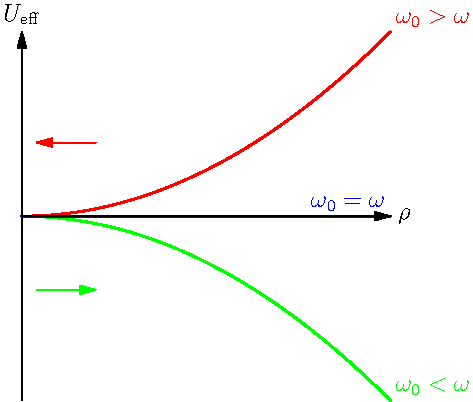
\includegraphics[width=\linewidth]{figures/Ueff.pdf}
\end{minipage}


\subsection{Discussion}
The total energy of the particle is given by 
\begin{align*}
E_0 = T + V = \frac{1}{2}m \left(\left(1 + 4\alpha^2 \rho^2\right) \dot{\rho}^2  + \omega^2\rho^2 \right) + mg \alpha \rho^2 = E + m\rho^2\omega^2.
\end{align*}
The conservation of $E$ implies $\dot{E}_0 = \dot{E} + 2 m \rho \dot{\rho} \omega^2 = 2 m \rho \dot{\rho} \omega^2$. From this, we see that $E_0$ is conserved on shell iff $\dot{\rho} = 0$ or $\rho = 0$. In the former case, $\rho$ is a constant and this can only be realised if $\omega_0=\omega$ or $\rho = 0$ (no effective force). In the latter case, $\rho = 0$ which is a subcase of $\dot{\rho}=0$. If $\omega_0<\omega$, the parabola is rotating fast enough to go beyond the gravitationnal pull of the particle towards $\rho=0$ and the velocity of the particle grows without bounds (the motor rotating the parabola is transfering energy to the particle and $E_0$ is not conserved). 
\pagebreak

\section{Brachistochrone}
Consider a particle subject to a uniform gravitationnal field of strength $g$ oriented in the negative $y$ direction of a planar $Oxy$ cartesian coordinate system. The particle starts at point $A$ of coordinates $x_A, y_A$ and ends at point $B$ of coordinates $x_B, y_B$. We are interested in the curve linking $A$ and $B$ minimizing the travel time of the particle. 
%\input{figures/P2_1.pdf}
\subsection{Travel time functionnal}
The first step in constructing the travel time functionnal is the parametrisation of its curve argument.  Suppose the trajectory is parametrised by $y$ so that it takes the form of a function $x(y)$. The length element at $x$ is $\text{d} l = \sqrt{\dot{x}(y)^2 + \dot{y}^2} \text{d} y = \sqrt{1 + \dot{x}(y)^2} \text{d} y$ with $\dot{()} = \frac{d}{dy}$. By a mass independant analogue of the conservation of energy $0 = \frac{1}{2} v^2-g y$ (with "potential" energy zero at $y_B$) where $v$ is the velocity, we have $v = \sqrt{2gy}$. For motion along an element $\text{d}l$ of the curve, the time elapsed is $\text{d}t = \text{d}l/\sqrt{2gy}$ leading to te following travel time functionnal 
\begin{align*}
    T[x(y)] = \int_{y_A}^{y_B} \text{d} y \dfrac{\sqrt{1 + \dot{x}(y)^2}}{\sqrt{2gy}}. 
\end{align*}

%If $x_A = x_B$, the trajectory has to be a straight vertical line. Indeed to minimize the travel time, gravity has to be exploited as much as possible and and disformation of the vertical path will reduce components of the gravitationnal acceleration along the trajectory (increasing the travel time). We therefore restrict the analysis to $x_B > x_A$.

%\input{figures/P1_1.pdf}
\subsection{Conserved quantity}
Since the integrand (effective lagrangian $L = \sqrt{1 + \dot{x}(y)^2}/{\sqrt{2gy}}$) of the previous functionnal is cyclic in $x$, the Euler-Lagrange equations imply 
\begin{align*}
    \dfrac{d}{dy}\left(\dfrac{\partial L}{\partial \dot{x}}\right) = 0 \implies Q = \dfrac{\partial L}{\partial \dot{x}} =\dfrac{2\dot{x}(y)}{\sqrt{1 + \dot{x}(y)^2}\sqrt{2gy}} \quad \text{is conserved on Brachistochrone}.
\end{align*}
We can now write 
\begin{align*}
    gy Q^2(1 + \dot{x}(y)^2) = 2\dot{x}(y)^2 &\implies \dot{x}(y) = \sqrt{\dfrac{gy Q^2}{2-gy Q^2}}\\ 
    &\implies x(y) = \int \text{d} y \sqrt{\dfrac{gy Q^2}{2-gy Q^2}} = \int \text{d} y \sqrt{\dfrac{gy Q^2}{2-gy Q^2}} 
\end{align*}



\newpage

\section{A sneaky recipe for the Noether charge}
%\input{figures/P3_1.pdf}
\subsection{Alternate Disformation}
Consider a particle described at time $t$ by the generalized coordinate $q(t)$ evolving with respect to a lagrangian $L$. A disformation of the particle's history is given by $q(t) \mapsto q' = q(t) +\epsilon \tilde{\delta}_s q(t)$ where $\delta \epsilon$ is an infinitesimal constant. This disformation contributes to the action $S$ with a boundary term if there exists a function $R_s$ such that $\tilde{\delta}_s L = \frac{d}{dt}R_s$ (first order variation of $L$ in $\epsilon$).
\subsection{Variation of the Action}
An alternative disformation of the history of the particle reads $q(t) \mapsto q'(t) = q(t) + \epsilon f(t) \tilde{\delta}_s q(t)$ where $f$ is a function vanishing at the start ($t=t_0$) and end ($t=t_1$) of the history. The action following from this disformation is 
\begin{align*}
    &S(q(t) +\epsilon f(t) \tilde{\delta}_s q(t))\\ &= \int_{t_0}^{t_1} \text{d}t \ L(q(t) +\epsilon f(t) \tilde{\delta}_s q(t), \dot{q}(t) +\epsilon \frac{d}{dt} (f(t) \tilde{\delta}_s q(t)), t) \\
    &= S(q(t))+\epsilon\int_{t_0}^{t_1} \text{d}t \left[\frac{\partial L}{\partial q}  f(t) \tilde{\delta}_s q(t) + \frac{\partial L}{\partial \dot{q}} (\dot{f}(t) \tilde{\delta}_s q(t)+f(t) \tilde{\delta}_s \dot{q}(t))\right] + O(\epsilon^2)\\
    &= S(q(t))+\epsilon\int_{t_0}^{t_1} \text{d}t \left[\frac{\partial L}{\partial q}  f(t) \tilde{\delta}_s q(t) -  \dfrac{d}{dt} \left(\frac{\partial L}{\partial \dot{q}} \tilde{\delta}_s q(t)\right) f(t)  + \frac{\partial L}{\partial \dot{q}} f(t) \tilde{\delta}_s \dot{q}(t) \right]  +  \left[\frac{\partial L}{\partial \dot{q}}   f(t) \tilde{\delta}_s q(t)\right]_{t_0}^{t_1}  + O(\epsilon^2)\\
    &= S(q(t))+\epsilon\int_{t_0}^{t_1} \text{d}t \left[\left(\frac{\partial L}{\partial q} \tilde{\delta}_s q(t)  + \frac{\partial L}{\partial \dot{q}} \tilde{\delta}_s \dot{q}(t)\right)  - \dfrac{d}{dt} \left(\frac{\partial L}{\partial \dot{q}} \tilde{\delta}_s q(t)\right)  \right] f(t)    + O(\epsilon^2)\\
    &= S(q(t))+\epsilon\int_{t_0}^{t_1} \text{d}t \left[\dfrac{d}{dt}R_s - \dfrac{d}{dt} \left(\frac{\partial L}{\partial \dot{q}} \tilde{\delta}_s q(t)\right)  \right] f(t) + O(\epsilon^2)
\end{align*}

and its first order variation reads $\delta_s^f S = -\int_{t_0}^{t_1} \text{d}t \dot{Q}_s f$ with $Q_s = \frac{\partial L}{\partial \dot{q}} \tilde{\delta}_s q(t) - R_s$. Using integration by parts we get 
\begin{align*}
    \delta_s^f S = \int_{t_0}^{t_1} \text{d}t \  Q_s \dot{f} + \left[\dot{Q}_s f\right]_{t_0}^{t_1} = \int_{t_0}^{t_1} \text{d}t \  Q_s \dot{f}.
\end{align*}
\subsection{Conserved quantity}
Since $f(t)\tilde{\delta}_s q(t)$ vanishes on the end points of the history, it can be interpreted the usual $\tilde{\delta} q(t)$ used in the action principle leading to on-shell histories. This means that teh first order variation of $S$ vanishes independently of $f$ on-shell. We have $0 = \delta_s^f S = -\int_{t_0}^{t_1} \text{d}t \dot{Q}_s f \implies \dot{Q}_s = 0$. Note that since $\dot{f}$ excludes constant functions except $f=0$, $\int_{t_0}^{t_1} \text{d}t \  Q_s \dot{f}$ can't be used to conclude $Q_s = 0$ ($\dot{f}$ is not arbitrary). 
\subsection{Application to time translations}
Consider the Lagrangian $L= m \dot{q}^2/2 - V(q)$ describing a particle of mass $m$ in a potential $V$. The infinitesimal disformation of an history due to time translation is given by $q'(t) = q(t+\epsilon) =  q(t) + \epsilon\dot{q}$ is associated to $\tilde{\delta}_s q = \dot{q}$. Here, we consider an altenrate disformation given by  $q'(t) = q(t+\epsilon) =  q(t) + f(t)\epsilon\dot{q}$ leading to the following variation of the action:
\begin{align*}
    &S(q(t) +\epsilon f(t) \tilde{\delta}_s q(t))\\ &= \int_{t_0}^{t_1} \text{d}t \ L(q(t) +\epsilon f(t) \tilde{\delta}_s q(t), \dot{q}(t) +\epsilon \frac{d}{dt} (f(t) \tilde{\delta}_s q(t)), t)
\end{align*}




% References
\makereferences
%-------------------------------------------------------


%%%%%%%%%%%%%%%%%%%%%%%%
% Terminer le document %
%%%%%%%%%%%%%%%%%%%%%%%%
\end{document}